\documentclass[a4paper, fleqn]{article}
\usepackage{header}

\pgfplotsset{compat=1.17}

\title{Семинарский лист 2.4}
\author{
    % Александр Богданов   \\ \href{https://t.me/SphericalPotatoInVacuum}{Telegram} \and
    % Алиса Вернигор       \\ \href{https://t.me/allisyonok}{Telegram} \and
     Анастасия Григорьева \\ \href{https://t.me/weifoll}{Telegram} \and
    % Василий Шныпко       \\ \href{https://t.me/yourvash}{Telegram} \and
    % Данил Казанцев       \\ \href{https://t.me/vserosbuybuy}{Telegram} \and
    Денис Козлов         \\ \href{https://t.me/DKozl50}{Telegram} \and
    Елизавета Орешонок   \\ \href{https://t.me/eaoresh}{Telegram} \and
    Ира Голобородько     \\ \href{https://t.me/Ira4kgl}{Telegram}
    % Иван Пешехонов       \\ \href{https://t.me/JohanDDC}{Telegram} \and
    % Иван Добросовестнов  \\ \href{https://t.me/ivankot13}{Telegram} \and
    % Настя Городилова     \\ \href{https://t.me/nastygorodi}{Telegram} \and
    % Никита Насонков      \\ \href{https://t.me/nnv_nick}{Telegram} \and
    % Сергей Лоптев        \\ \href{https://t.me/beast_sl}{Telegram}
}

\date{Версия от {\ddmmyyyydate\today} \currenttime}

\begin{document}
    \maketitle
   
    \section*{Предполагая функцию $f$ непрерывной на $D$, запишите тройной интеграл от $f$ по $D$ в виде
    одного из повторных, если $D$ задано неравенствами.}
    
    \subsection*{Задача 1} 
    
    $0 \leq z \leq 4 - x^2, \; x^2 - y^2 \geq 0, \; x \geq 0. $
    
    Хочу интегрировать в порядке $\displaystyle \int \limits_{\dots}^{\dots} dx \int \limits_{\dots}^{\dots} dy \int \limits_{\dots}^{\dots} f(x, y, x) dz.$
    
    Посмотрим, что происходит при фиксированном $x$.
    
    Так как $x^2 \geq y^2 \iff |x| \geq |y|,$ то $-x \leq y \leq x \;  $ ($x$ положительный). Ещё знаем, что $0 \leq z \leq 4 -x^2.$
    
    Итак,  $\displaystyle \int \limits_{\dots}^{\dots} dx \int \limits_{-x}^{x} dy \int \limits_{0}^{4 -x^2} f(x, y, x) dz.$ 
    
    А каковы границы $x$? $x \geq 0$, это нам дано. Из того, что $z \in [0, 4 -x^2]$, сделаем вывод, что $x \leq 2$, ведь при больших значениях $x$ множество становится вырожденным.
    
    Так что границы интегрирования знаем,  $\boxed{\displaystyle \int \limits_{0}^{2} dx \int \limits_{-x}^{x} dy \int \limits_{0}^{4 -x^2} f(x, y, x) dz} \; .$ 
    
    
    \subsection*{Задача 2}
    \begin{flalign*}
        & x + y + z \leq 2; \;\; 0 \leq 4z \leq 4 - x^2 - y^2; \;\; x \geq 0; \;\; y \geq 0 \\
        & \begin{cases} 
            x \geq 0, \;\; y \geq 0; \;\; z \geq 0 \\
            x + y + z \leq 2 \\
            x^2 + y^2 \leq 4 - 4z 
        \end{cases} \Rightarrow \begin{cases} 
            x \in [0, 2] \\
            y \in [0, 2] \\
            z \in [0, 1]
        \end{cases} \\
        & \begin{cases} 
            z = 2 - x - y \\
            4z = 4 - x^2 - y^2 
        \end{cases} \implies \;\; 8 - 4x - 4y = 4 - x^2 - y^2 \Rightarrow y = \sqrt{4x - x^2} + 2 \text{ — пересечение фигур} \\
        & \int\limits_{0}^1 dx \left\{ 
            \int\limits_0^{\sqrt{4x - x^2} + 2} dy \int\limits_0^{1 - \frac{x^2}{4} - \frac{y^2}{4}} f(x, y, z) dx + 
            \int\limits_{\sqrt{4x - x^2}+2}^{1-x} dy \int\limits_{0}^{2-x-y} f(x, y, z) dz
        \right\} 
    \end{flalign*}
    
    Пересечение параболоида и плоскости. Первый интеграл отвечает за часть параболоида, а второй — за плоскость.

    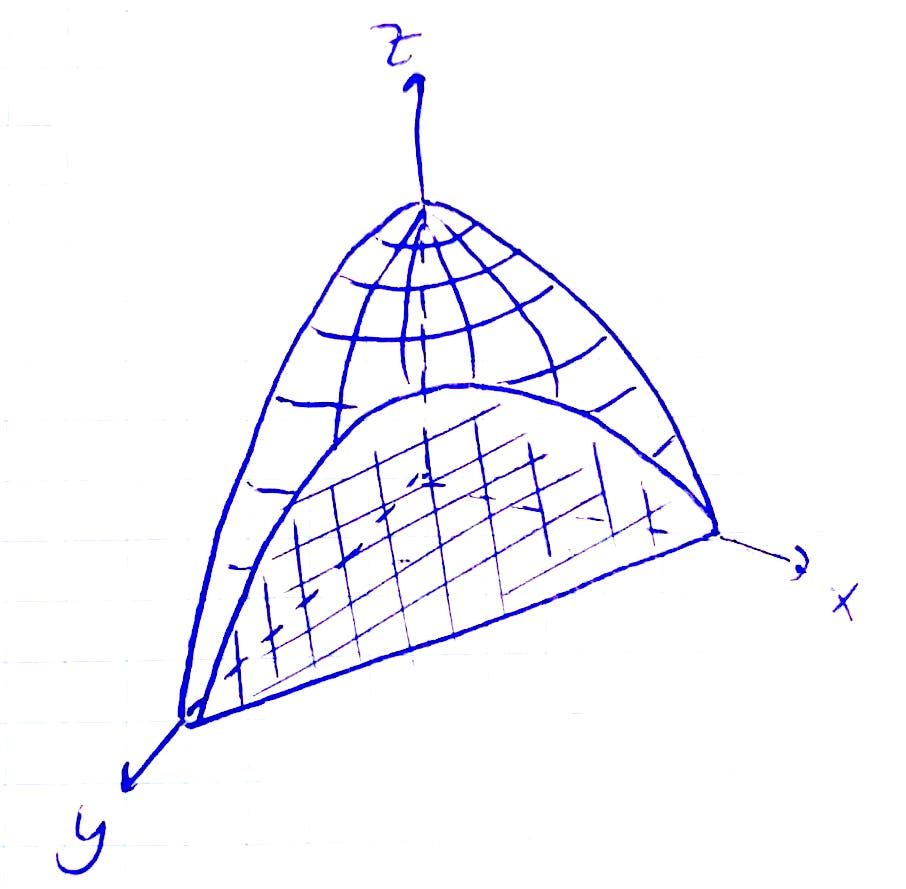
\includegraphics[width=6cm]{./list24imgs/task2.jpg}
    
    
    \subsection*{Задача 3}
    
    $0 \leq z \leq 4xy, \; x + 4y + z \leq 1. $
    
    Буду интегрировать $\displaystyle \int \limits_{\dots}^{\dots} dx \int \limits_{\dots}^{\dots} dy \int \limits_{\dots}^{\dots} f(x, y, x) dz.$
    
    Для невырожденности $D$ требуется $\begin{cases} x \neq 0; \\ y \neq 0. \end{cases}$
    
    Из того, что $0 \leq xy$, делаем вывод, что $x$  и $y$ одного знака.
    
    \textit{Случай I.} $\begin{cases} x > 0; \\ y > 0. \end{cases}$
    
    При фиксированном $x$ в срезе $Oyz$ нас интересуют точки треугольника, ограниченного прямыми $z = 4xy$, $z = -4y - x + 1$ и $z = 0$.
    
   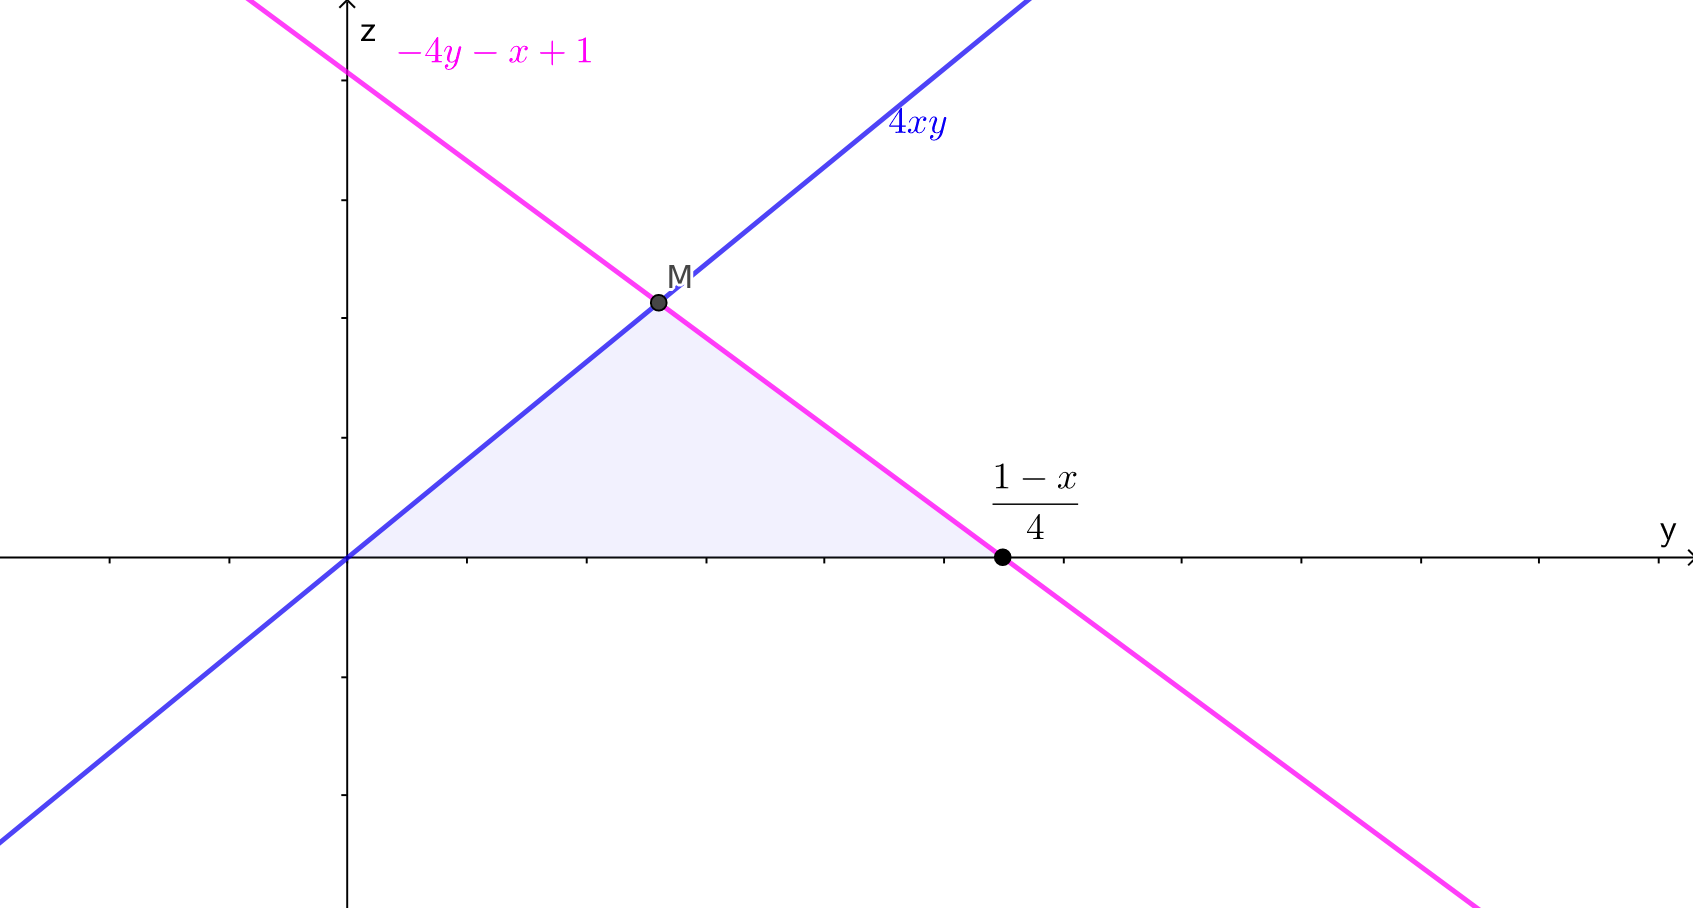
\includegraphics[width=12cm, height=7cm]{list24imgs/task 2.4.5.png}
   
   Найдём $y$-координату точки $M$: $ -4y -x + 1 = 4xy \implies 4y(x + 1) = 1 - x \implies M_y = \frac{1 - x}{4x  + 4}.$
   
   Множество является вырожденным, т. и т.т. прямая $z = -4y - x + 1$ проходит через $0$, т.е. при $x = 1.$
   
   Значит, в данном случае $x \in (0, 1)$. Интегрируем!
   
   $\displaystyle \int \limits_{0}^{1} dx \left( \int \limits_{0}^{M_y} dy \int \limits_{0}^{4xy} f \,  dz + \int \limits_{M_y}^{(1 - x)/4} dy \int \limits_{0}^{-4y - x + 1} f \,  dz \right), \; $ где  $M_y = \frac{1 - x}{4x  + 4}$.
   
   \textit{Случай II.} $\begin{cases}
   x < 0;\\
   y < 0.
   \end{cases}$
   
   При фиксированном $x$ в срезе $Oyz$ происходит такая жуть:
   
   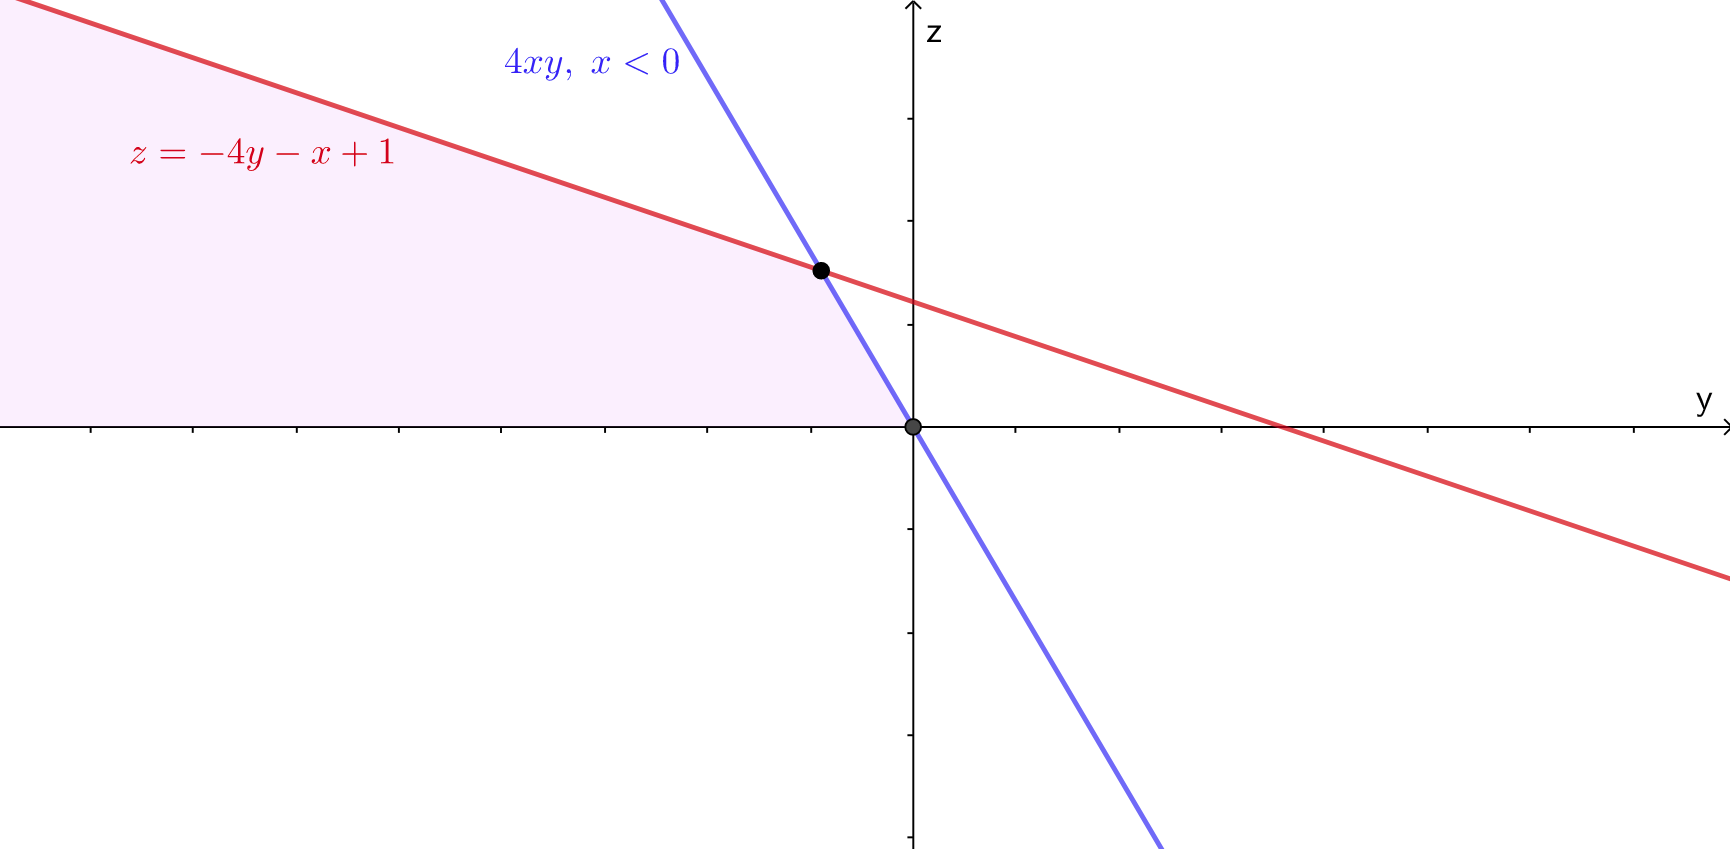
\includegraphics[width=13cm, height=7cm]{list24imgs/task 2.4.5-2.png}
    
    Данная область неограничена снизу по $y$, значит она бесконечная $\implies$ интеграл от неё невозможно взять.
    
    \subsection*{Задача 4}
    
    $y^2 \le z \le 4, \; x^2 + y^2 \le 16$\\
    
    Все точки рассматриваемой области находятся внутри круга радиуса 4 с центром в начале координат (его задает неравенство $x^2 + y^2 \le 16$). Значения $z$, как видно из 1-го неравенства, лежат в промежутке $[y^2; 4]$. Искомый повторный интеграл может иметь вид:
    \[ \int\limits_{-4}^{4} dx \int\limits_{-\sqrt{16-x^2}}^{\sqrt{16-x^2}} dy \int\limits_{y^2}^{4} f(x, y, z)\, dz  \]
    
    \subsection*{Задача 5}
    
    $x^2 + y^2 \geq 3 z^2, \; x^2 + y^2 - z^2 \leq 2. $
    
    Проинтегрируем внешне по $z$. 
    
    $z = const \implies x^2 + y^2 \geq 3z^2, \; x^2 + y^2 \leq z^2 + 2.$
    
    Нам интересно примерно такое колечко:
    
    
   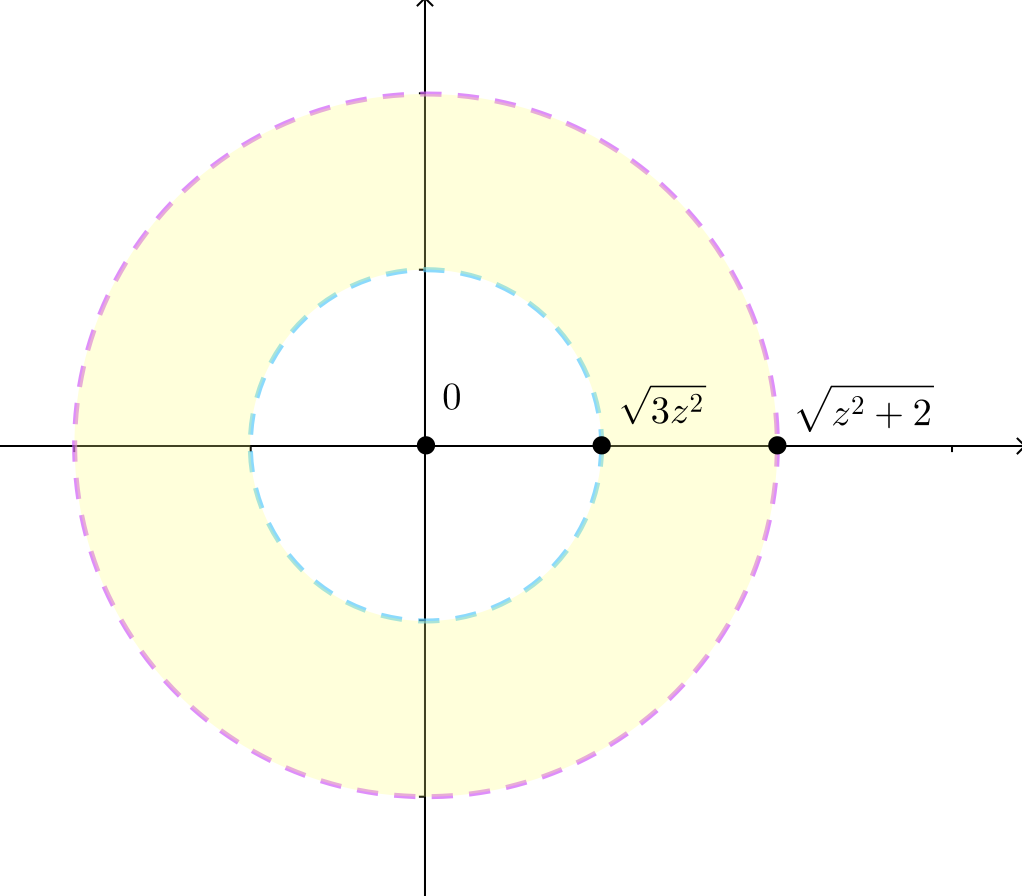
\includegraphics[width=8.5cm, height=8cm]{list24imgs/task 2.4.3.png}
    
    Можно начать разбивать область интегрирования по $x$. Но мы ленивые. Поэтому просто вычтем из площади большей окружности площадь меньшей.
    
    Тогда внутри интеграла по $z$ появится $\displaystyle \int \limits_{-\sqrt{z^2 + 2}}^{\sqrt{z^2 + 2}} dx \int \limits_{-\sqrt{z^2 + 2 - x^2}}^{\sqrt{z^2 + 2 - x^2}} f dy - \int \limits_{-\sqrt{3z^2}}^{\sqrt{3z^2}} dx \int \limits_{-\sqrt{3z^2- x^2}}^{\sqrt{3z^2 - x^2}} f dy  .$
    
    
    Для не-вырожденности множества, получаем условие $\sqrt{3z^2} \leq \sqrt{z^2 + 2} \iff 2z^2 \leq 2 \iff |z| \leq 1 \iff z \in [-1, 1].$
    
    
    Итого $\displaystyle \int \limits_{-1}^{1} dz \left( \; \int \limits_{-\sqrt{z^2 + 2}}^{\sqrt{z^2 + 2}} dx \int \limits_{-\sqrt{z^2 + 2 - x^2}}^{\sqrt{z^2 + 2 - x^2}} f dy - \int \limits_{-\sqrt{3z^2}}^{\sqrt{3z^2}} dx \int \limits_{-\sqrt{3z^2- x^2}}^{\sqrt{3z^2 - x^2}} f dy  \right).$
    
    \subsection*{Задача 6}
    
    $y^2 + x + z \le 1, \; x \ge z \ge 0$
    
    Проинтегрируем в порядке \\[3 pt]
    $\int\limits_{\dots}^{\dots} dy \int\limits_{\dots}^{\dots} dx \int\limits_{\dots}^{\dots} f(x, y, z)\, dz$ \\
    
    При фиксированном $y$ неравенства $y^2 + x + z \le 1$ и $x \ge z \ge 0$ можно переписать в виде системы
    \[ \left\{\begin{array}{rcl} z &\le& (1-y^2) - x, \\ z &\le& x, \\ z &\ge& 0 \end{array}\right., \]
    задающей треугольник, ограниченный прямыми $z = (1-y^2)-x$, $z = x$ и $z = 0$, при условии того, что точка пересечения прямых $z = (1-y^2)-x$ и $z = x$ находится не ниже оси $Ox$:
    \[ (1-y^2)-x = x \Leftrightarrow x = \frac{1-y^2}2 \Rightarrow z = x = \frac{1-y^2}2 \ge 0 \Rightarrow 1-y^2 \ge 0 \Leftrightarrow y \in [-1; 1] \]
    
    Значения $x$ нас интересуют только те, при которых $z \ge 0 \Leftrightarrow \left\{\begin{array}{rcl} (1-y^2)-x &\ge& 0, \\ x &\ge& 0 \end{array}\right. \Leftrightarrow \left\{\begin{array}{rcl} x &\le& (1-y^2), \\ x &\ge& 0 \end{array}\right.$, \\[3 pt]
    т.е. $x \in [0; 1-y^2]$. При этом при $x \le \frac{1-y^2}2$ значения $z$ лежат на отрезке $[0; x]$, а при $x \ge \frac{1-y^2}2$ --- на отрезке $[0; 1-y^2]$ \\
    
    Получили границы для повторного интеграла:
    \[ \int\limits_{-1}^{1} dy \left( \int\limits_{0}^{\frac{1-y^2}2} dx \int\limits_{0}^{x} f(x, y, z)\, dz + \int\limits_{\frac{1-y^2}2}^{1-y^2} dx \int\limits_{0}^{1-y^2} f(x, y, z)\, dz \right) \]
    
    \section*{Вычислите интеграл.}
    \subsection*{Задача 7} 
    $\displaystyle \int\limits_{0}^{1} dx  \int\limits_{0}^{x} dy \int \limits_{0}^{xy} (x + y + z) dz = \int\limits_{0}^{1} dx  \int\limits_{0}^{x} dy \left( \int \limits_{0}^{xy} (x) dz +  \int \limits_{0}^{xy} (y) dz + \int \limits_{0}^{xy} (z) dz \right) = 
    \int\limits_{0}^{1} dx  \int\limits_{0}^{x} dy \left( x \int  \limits_{0}^{xy} 1 \, dz +  y \int \limits_{0}^{xy} 1 \, dz + \int \limits_{0}^{xy} (z) dz \right) = \\
    = \int\limits_{0}^{1} dx  \int\limits_{0}^{x} dy \left(x \cdot (xy) + y \cdot (xy) +  \frac{(xy)^2}{2} \right) =   \int\limits_{0}^{1} x \, dx  \cdot \int\limits_{0}^{x} dy  \left( xy + y^2  +  \frac{xy^2}{2} \right)  =
    \int\limits_{0}^{1} x \cdot \left( x \cdot \left( \frac{x^2}{2}\right) + \frac{x^3}{3} + x \cdot \left(\frac{x^3}{6} \right)\right) dx  = \\ = \int\limits_{0}^{1} \frac{x^4}{2} + \frac{x^4}{3} + \frac{x^5}{6}  dx  = \left(\frac{x^5}{10} + \frac{x^5}{15} + \frac{x^6}{36} \Bigg|_0^1\right) = \frac{1}{10} + \frac{1}{15} + \frac{1}{36} = \frac{3 + 2}{30} + \frac{1}{36} = \frac{6}{36} + \frac{1}{36} = \frac{7}{36}. $
    
    \subsection*{Задача 8}
    \begin{flalign*}
        & \int\limits_{1}^{2} dy \int\limits_{y}^{2} dx \int\limits_{0}^{1/(xy)} \frac{dz}{x(1 + x^2 y^2 z^2)}
        = \left[\, u = xyz, \, \frac{du}{dz} = xy \Leftrightarrow dz = \frac{du}{xy} \,\right] 
        \; \int\limits_{1}^{2} dy \int\limits_{y}^{2} \frac1x\cdot\frac1{xy}\,dx \int\limits_{0}^{1} \frac{du}{1 + u^2} = \\
        & = \int\limits_{1}^{2} dy \int\limits_{y}^{2} \frac1x\cdot\frac1{xy}\,dx \cdot \left( \arctg u \Bigm|_{0}^{1} \right)
        = \frac{\pi}4\, \int\limits_{1}^{2} \frac1y\, dy \int\limits_{y}^{2} \frac1{x^2}\,dx 
        = \frac{\pi}4\, \int\limits_{1}^{2} \frac1y\, dy \cdot \left( -\frac1x \Bigm|_{y}^{2} \right)
        = \frac{\pi}4\, \int\limits_{1}^{2} \frac1y\left( \frac1y-\frac12 \right)\, dy = \\
        & = \frac{\pi}4\, \left( \int\limits_{1}^{2} \frac1{y^2}\, dy - \frac12\,\int\limits_{1}^{2} \frac1{y}\, dy \right) 
        = \frac{\pi}4\, \left( -\frac1y \Bigm|_{1}^{2} - \frac12\,\ln y \Bigm|_{1}^{2} \right)
        = \frac{\pi}4\, \left( 1-\frac12 - \frac12\,\ln 2 \right) = \frac{\pi}8\, (1 - \ln2) \\
    \end{flalign*}
    
    \subsection*{Задача 9}    
    $\displaystyle \int\limits_{0}^{4} dz \int \limits_{-z}^{z} dx \int \limits_{0}^{\sqrt{z^2 - x^2}} z^2 x y^2 dy.$
    
    Для удобства, хочу проинтегрировать в порядке $z-y-x.$ Чтобы поменять $x$ и $y$ местами, рассмотрю срез $D$ при произвольном фиксированном $z = z_0.$
    
    $x \in [-z_0, z_0]$, точки $D$ лежат в половинке окружности радиуса $z_0$ выше нуля.
    
    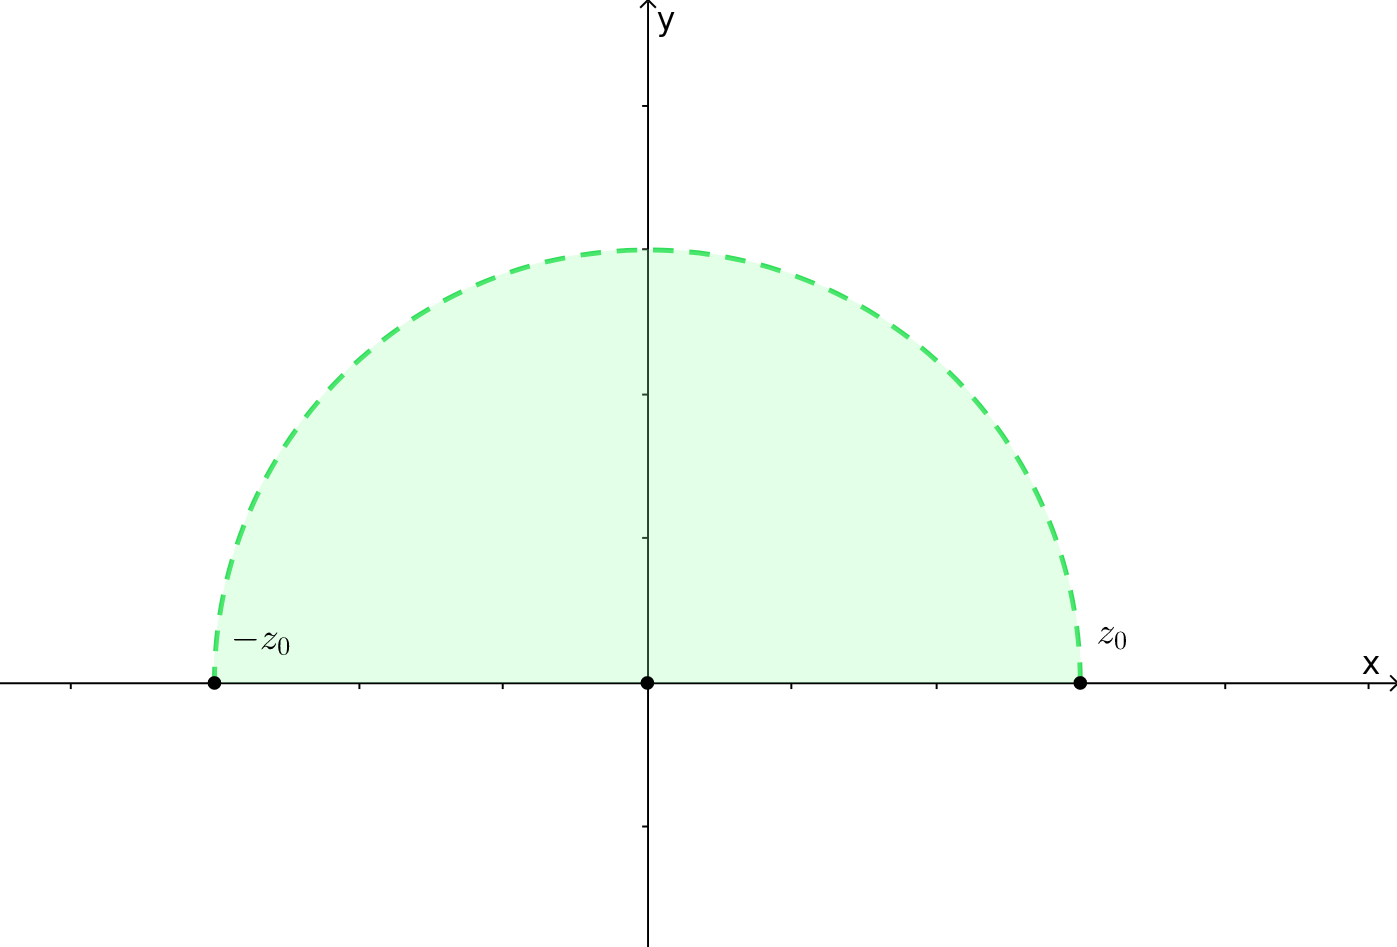
\includegraphics[width=12cm, height=8cm]{list24imgs/task 2.4.9.png}
    
    Если изменим порядок интегрирования, то $y \in [0, z]$, $\; \; x \in \left[-\sqrt{z^2 - y^2}, \sqrt{z^2 - y^2}\right]$
    
    $\displaystyle \int\limits_{0}^{4} dz \int \limits_{0}^{z} dy \int \limits_{0}^{\sqrt{z^2 - y^2}} z^2 x y^2 dx = \displaystyle \int\limits_{0}^{4} z^2  dz \int \limits_{0}^{z} y^2  dy \int \limits_{-\sqrt{z^2 - y^2}}^{\sqrt{z^2 - y^2}} x \, dx = \int\limits_{0}^{4} z^2  dz \int \limits_{0}^{z} y^2  dy \left( \frac{x^2}{2} \Bigg|_{-\sqrt{z^2 - y^2}}^{\sqrt{z^2 - y^2}} \right) = 0.$
    
    
    \subsection*{Задача 10}
    \begin{flalign*}
        & \int\limits_{1}^{3} dz \int\limits_{1-z}^{3-z} dy \int\limits_{0}^{3-y-z} \frac{dx}{(x + y + z)^2}
        = \left[\, u = x+y+z, \, \frac{du}{dx} = 1 \Leftrightarrow dx = du \,\right] 
        \; \int\limits_{1}^{3} dz \int\limits_{1-z}^{3-z} dy \int\limits_{y + z}^{3} \frac{du}{u^2} = \\
        & = \int\limits_{1}^{3} dz \int\limits_{1-z}^{3-z} dy \cdot \left( -\frac1u \Bigm|_{y+z}^{3} \right)
        = \int\limits_{1}^{3} dz \int\limits_{1-z}^{3-z} \left( \frac1{y+z}-\frac13 \right)dy
        = \left[\, v = y+z, \, dy = dv \,\right] \: \int\limits_{1}^{3} dz \left( \:\int\limits_{1}^{3} \frac1{v}\,dv - \frac13\int\limits_{1-z}^{3-z}dy \right) = \\
        & = \int\limits_{1}^{3} dz \left( \ln3 - \frac13\,((3-z) - (1-z)) \right) 
        = \int\limits_{1}^{3} dz \left( \ln3 - \frac23 \right) = \left( \ln3 - \frac23 \right)(3-1) = 2\ln3-\frac43 \\
    \end{flalign*}
    
    \section*{Измените порядок интегрирования и вычислите интеграл.}
    
    \subsection*{Задача 11}
    $\displaystyle \int\limits_{0}^{\sqrt[3]{\pi}} dx \int\limits_{x}^{\sqrt[3]{\pi}} dy
    \int\limits_{y}^{\sqrt[3]{\pi}}\sin (z^3) dz.$ Исследуем границы для восстановления $D$.
    
    $x \in [0, \sqrt[3]{\pi}].$ Нам интересны точки между плоскостями $x = y$ и $y = \sqrt[3]{\pi}$. 
    
    Вертикально множество ограничено плоскостями $y = z$ и $z = \sqrt[3]{\pi}.$ Итого получили пирамидку:
    
    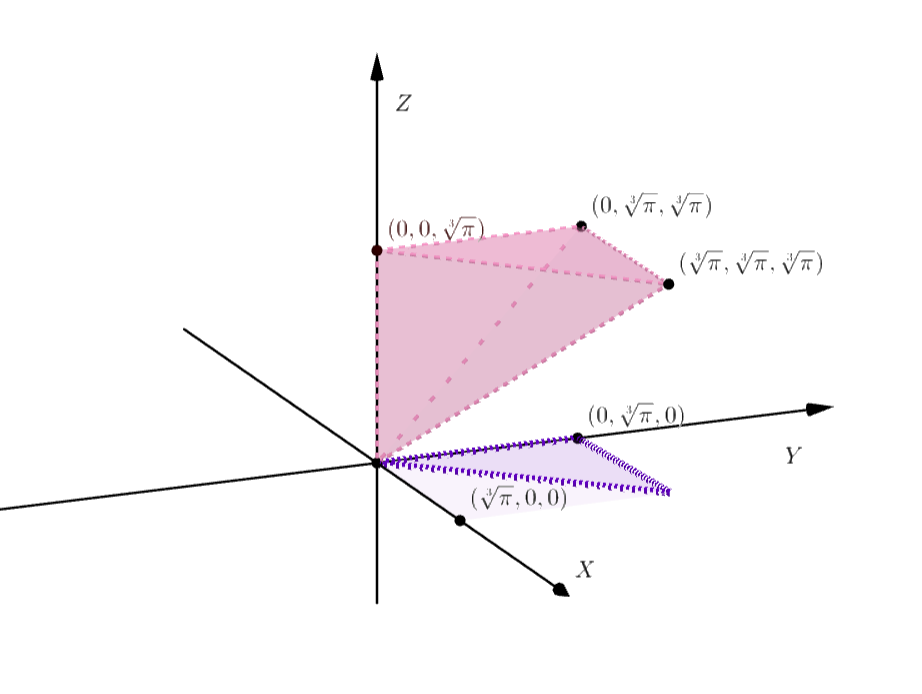
\includegraphics[width=12cm, height=10cm]{list24imgs/task 2.4.11.png}        
    
    Так как функция зависит от $z$, то сначала лучше интегрировать именно по $z$. 
    
    $\displaystyle \int \limits_{0}^{\sqrt[3]{\pi}} \sin (z^3) dz \int \limits_{0}^{z} dy
    \int \limits_{0}^{y} dx = 
     \int \limits_{0}^{\sqrt[3]{\pi}} \sin (z^3) dz \int \limits_{0}^{z} y \; dy = 
     \int \limits_{0}^{\sqrt[3]{\pi}}  \frac{z^2}{2} \cdot \sin (z^3) dz = \left[ t = z^3; \; dt = 3z^2dz \right] =  
     \frac{1}{6} \cdot \int \limits_{0}^{\pi}    \sin t \, dt = \frac{1}{6} \left( -\cos t \Bigg|_{0}^{\pi}\right) = \\ = \frac{1}{6} + \frac{1}{6} = \boxed{\frac{1}{3}} \, .$
    
    
    \subsection*{Задача 12}
    \begin{flalign*}
        & \int_0^1 dx \int_x^1 dy \int_y^1 e^{z^3} dz = 
        \int_0^1 e^{z^3} dz \int_0^z dy \int_0^y dx = 
        \int_0^1 e^{z^3} dz \int_0^z y dy = 
        \int_0^1 \frac{z^2}{2} e^{z^3} dz = \left\{ \begin{array} {rl}
            u = & z^3 \\
            du = & 3z^2 dz \\
            dz = & \frac{du}{3z^2} 
        \end{array} \right\} = \\
        & = \int_0^1 \frac{1}{6} e^u du = \frac{e - 1}{6} 
    \end{flalign*}
    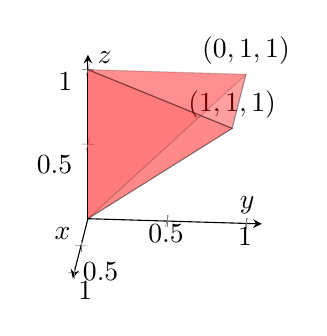
\begin{tikzpicture} 
        \begin{axis} [width=6cm, xlabel={$x$}, ylabel={$y$}, zlabel={$z$}, axis lines=center, axis equal image,
                        view={95}{20}, clip=false,
                        xmin=0, xmax=1.1, ymin=0, ymax=1.1, zmin=0, zmax=1.1]
            \coordinate (O) at (axis cs:0, 0, 0);
            \coordinate[label=above:{$(1, 1, 1)$}] (A) at (axis cs:1, 1, 1);
            \coordinate (B) at (axis cs:0, 0, 1);
            \coordinate[label=above:{$(0, 1, 1)$}] (C) at (axis cs:0, 1, 1); 
            
            \draw[fill=red, opacity=0.1] (O) -- (A) -- (C); 
            \draw[fill=red, opacity=0.4] (O) -- (A) -- (B); 
            \draw[fill=red, opacity=0.2] (O) -- (C) -- (B); 
            \draw[fill=red, opacity=0.3] (C) -- (A) -- (B); 
        \end{axis} 
    \end{tikzpicture} 

    
    \subsection*{Задача 13}

    $\displaystyle \int\limits_{0}^{1} dx \int\limits_{x}^{1} dy \int\limits_{y}^{1} \frac{\arctg z}{z} dz.$

    Чтобы было удобнее, сделаем первым интегралом $z$. Для этого сначала поменяем $y$ и $z$, а потом $z$ и $x$. 

    $y \leftrightarrow z.$ При фиксированном $x$ такая ситуация:

    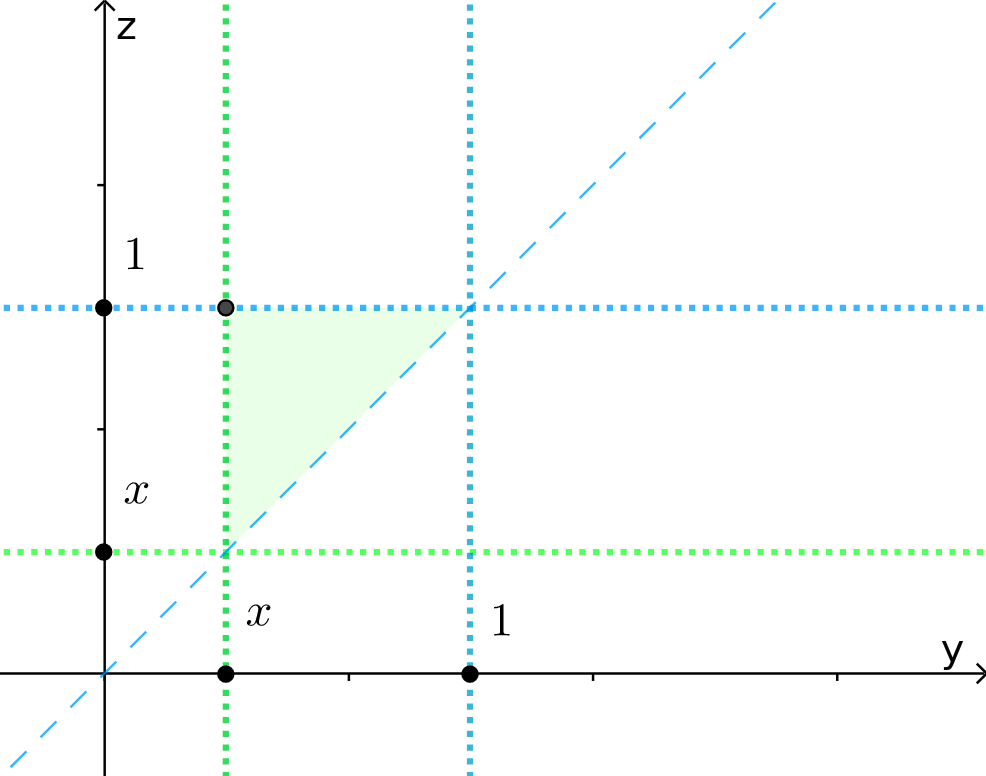
\includegraphics[width=7cm, height=6cm]{list24imgs/task 2.4.13-1.png}

    Значит, поменяв порядок  $y$ и $z$, получим $\displaystyle \int\limits_{0}^{1} dx \int\limits_{x}^{1} dz \int\limits_{x}^{z} \frac{\arctg z}{z} dy.$

    Теперь меняем местами $x$ и $z$. Смотрим, что происходит с $z$ в зависимости от $x$:

    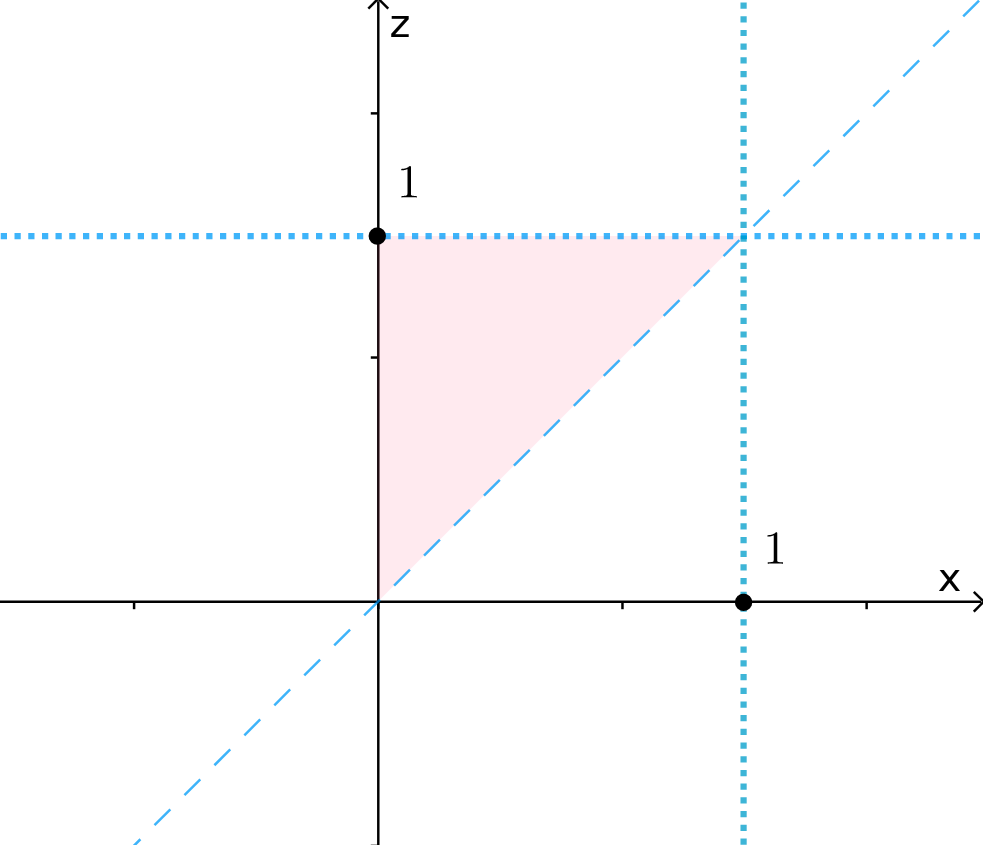
\includegraphics[width=7cm, height=6cm]{list24imgs/task 2.4.13-2.png}

    Итого выйдет $\displaystyle \int\limits_{0}^{1} dz \int\limits_{0}^{z} dx \int\limits_{x}^{z} \frac{\arctg z}{z} dy = \int\limits_{0}^{1} dz \int\limits_{0}^{z}  \frac{\arctg z}{z}  dx \int\limits_{x}^{z}  dy = \int\limits_{0}^{1} dz \int\limits_{0}^{z}  (z - x)\frac{\arctg z}{z}  dx  = \int\limits_{0}^{1} \arctg z \, dz \int\limits_{0}^{z}  1 - \frac{x}{z}  \, dx = \\ = \int\limits_{0}^{1} \left(z - \frac{z^2}{2z} \right)\arctg z \, dz = \int\limits_{0}^{1} \frac{z}{2} \arctg z \, dz = \frac{1}{2} \int\limits_{0}^{1} z \arctg z \, dz.$

     Интегрируем по частям: $\begin{cases} f = \frac{z^2}{2}; \; df = zdz; \\
     g  = \arctg z; \; dg = \frac{1}{1 + z^2} dz.
     \end{cases}$

     Тогда $\int\limits_{0}^{1} z \arctg z \, dz = \int\limits_{0}^{1} g \, df = \left( fg \,  \Bigg|_{0}^{1} \right) - \int\limits_{0}^{1} fdg =  \left( \frac{z^2}{2} \cdot \arctg z \Bigg|_{0}^{1} \right) - \int\limits_{0}^{1} \frac{z^2}{2(1 + z^2)} dz = \\ = \frac{\pi}{8} -  \frac{1}{2} \left(\int\limits_{0}^{1} \frac{1 + z^2}{1 + z^2} dz -  \int\limits_{0}^{1} \frac{1}{(1 + z^2)} dz\right) = \frac{\pi}{8} - \frac{1}{2} + \frac{1}{2} \arctg(1) = \frac{\pi}{8} - \frac{1}{2} + \frac{\pi}{8} = \frac{\pi}{4} - \frac{1}{2}.$ 

     Не забываем домножить всё это дело на $\frac{1}{2}$, и получаем ответ, $\boxed{\frac{\pi}{8} - \frac{1}{4}} \, .$

    % \subsection*{Задача 14}
    
    % \subsection*{Задача 15}
    
    % \subsection*{Задача 16}
    
    % \subsection*{Задача 17}
    
    \section*{Вычислите многократный интеграл.}
    % \subsection*{Задача 18}
    
    % \subsection*{Задача 19}
    
    % \subsection*{Задача 20}
    
    % \subsection*{Задача 21}
    
    % \subsection*{Задача 22}
    
    % \subsection*{Задача 23}
    
\end{document}
